\documentclass[1p]{elsarticle_modified}
%\bibliographystyle{elsarticle-num}

%\usepackage[colorlinks]{hyperref}
%\usepackage{abbrmath_seonhwa} %\Abb, \Ascr, \Acal ,\Abf, \Afrak
\usepackage{amsfonts}
\usepackage{amssymb}
\usepackage{amsmath}
\usepackage{amsthm}
\usepackage{scalefnt}
\usepackage{amsbsy}
\usepackage{kotex}
\usepackage{caption}
\usepackage{subfig}
\usepackage{color}
\usepackage{graphicx}
\usepackage{xcolor} %% white, black, red, green, blue, cyan, magenta, yellow
\usepackage{float}
\usepackage{setspace}
\usepackage{hyperref}

\usepackage{tikz}
\usetikzlibrary{arrows}

\usepackage{multirow}
\usepackage{array} % fixed length table
\usepackage{hhline}

%%%%%%%%%%%%%%%%%%%%%
\makeatletter
\renewcommand*\env@matrix[1][\arraystretch]{%
	\edef\arraystretch{#1}%
	\hskip -\arraycolsep
	\let\@ifnextchar\new@ifnextchar
	\array{*\c@MaxMatrixCols c}}
\makeatother %https://tex.stackexchange.com/questions/14071/how-can-i-increase-the-line-spacing-in-a-matrix
%%%%%%%%%%%%%%%

\usepackage[normalem]{ulem}

\newcommand{\msout}[1]{\ifmmode\text{\sout{\ensuremath{#1}}}\else\sout{#1}\fi}
%SOURCE: \msout is \stkout macro in https://tex.stackexchange.com/questions/20609/strikeout-in-math-mode

\newcommand{\cancel}[1]{
	\ifmmode
	{\color{red}\msout{#1}}
	\else
	{\color{red}\sout{#1}}
	\fi
}

\newcommand{\add}[1]{
	{\color{blue}\uwave{#1}}
}

\newcommand{\replace}[2]{
	\ifmmode
	{\color{red}\msout{#1}}{\color{blue}\uwave{#2}}
	\else
	{\color{red}\sout{#1}}{\color{blue}\uwave{#2}}
	\fi
}

\newcommand{\Sol}{\mathcal{S}} %segment
\newcommand{\D}{D} %diagram
\newcommand{\A}{\mathcal{A}} %arc


%%%%%%%%%%%%%%%%%%%%%%%%%%%%%5 test

\def\sl{\operatorname{\textup{SL}}(2,\Cbb)}
\def\psl{\operatorname{\textup{PSL}}(2,\Cbb)}
\def\quan{\mkern 1mu \triangleright \mkern 1mu}

\theoremstyle{definition}
\newtheorem{thm}{Theorem}[section]
\newtheorem{prop}[thm]{Proposition}
\newtheorem{lem}[thm]{Lemma}
\newtheorem{ques}[thm]{Question}
\newtheorem{cor}[thm]{Corollary}
\newtheorem{defn}[thm]{Definition}
\newtheorem{exam}[thm]{Example}
\newtheorem{rmk}[thm]{Remark}
\newtheorem{alg}[thm]{Algorithm}

\newcommand{\I}{\sqrt{-1}}
\begin{document}

%\begin{frontmatter}
%
%\title{Boundary parabolic representations of knots up to 8 crossings}
%
%%% Group authors per affiliation:
%\author{Yunhi Cho} 
%\address{Department of Mathematics, University of Seoul, Seoul, Korea}
%\ead{yhcho@uos.ac.kr}
%
%
%\author{Seonhwa Kim} %\fnref{s_kim}}
%\address{Center for Geometry and Physics, Institute for Basic Science, Pohang, 37673, Korea}
%\ead{ryeona17@ibs.re.kr}
%
%\author{Hyuk Kim}
%\address{Department of Mathematical Sciences, Seoul National University, Seoul 08826, Korea}
%\ead{hyukkim@snu.ac.kr}
%
%\author{Seokbeom Yoon}
%\address{Department of Mathematical Sciences, Seoul National University, Seoul, 08826,  Korea}
%\ead{sbyoon15@snu.ac.kr}
%
%\begin{abstract}
%We find all boundary parabolic representation of knots up to 8 crossings.
%
%\end{abstract}
%\begin{keyword}
%    \MSC[2010] 57M25 
%\end{keyword}
%
%\end{frontmatter}

%\linenumbers
%\tableofcontents
%
\newcommand\colored[1]{\textcolor{white}{\rule[-0.35ex]{0.8em}{1.4ex}}\kern-0.8em\color{red} #1}%
%\newcommand\colored[1]{\textcolor{white}{ #1}\kern-2.17ex	\textcolor{white}{ #1}\kern-1.81ex	\textcolor{white}{ #1}\kern-2.15ex\color{red}#1	}

{\Large $\underline{12n_{0383}~(K12n_{0383})}$}

\setlength{\tabcolsep}{10pt}
\renewcommand{\arraystretch}{1.6}
\vspace{1cm}\begin{tabular}{m{100pt}>{\centering\arraybackslash}m{274pt}}
\multirow{5}{120pt}{
	\centering
	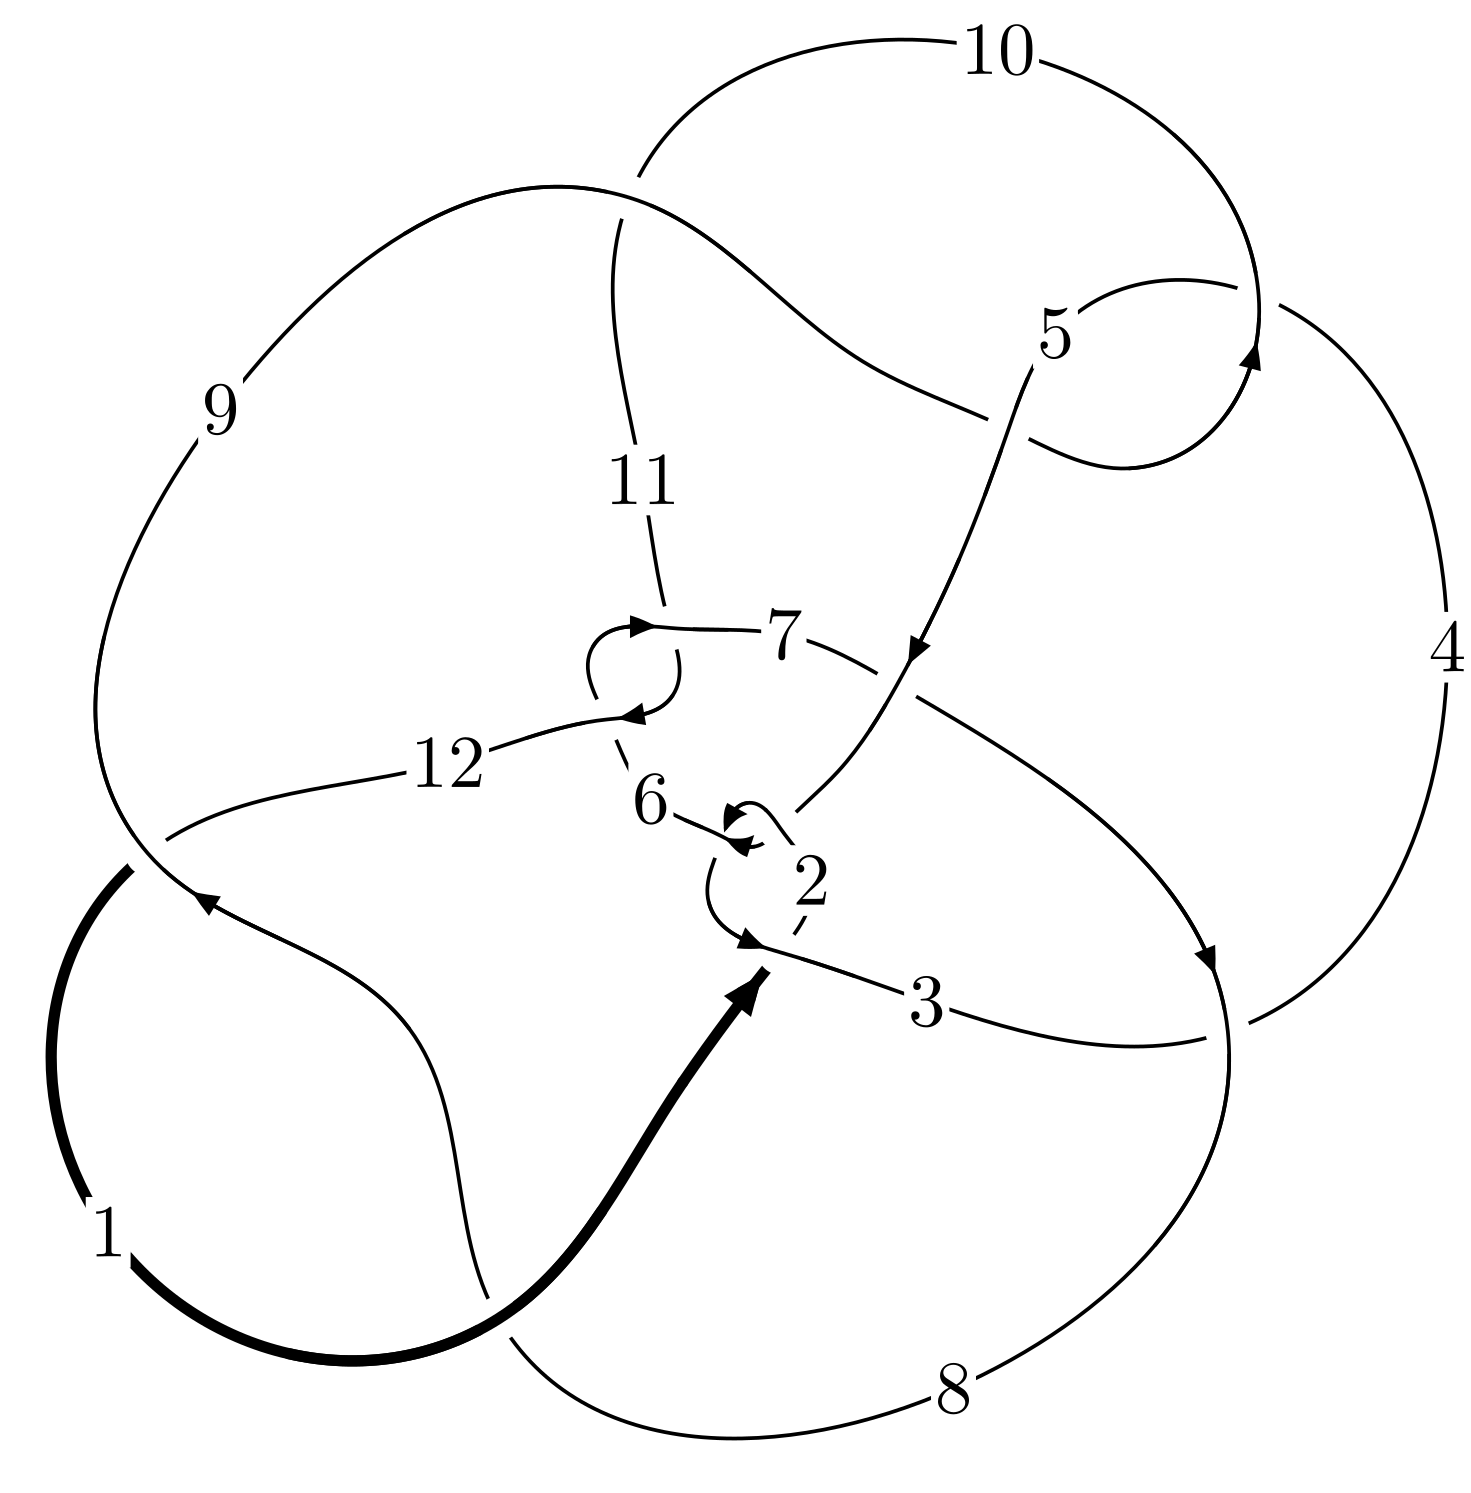
\includegraphics[width=112pt]{../../../GIT/diagram.site/Diagrams/png/2472_12n_0383.png}\\
\ \ \ A knot diagram\footnotemark}&
\allowdisplaybreaks
\textbf{Linearized knot diagam} \\
\cline{2-2}
 &
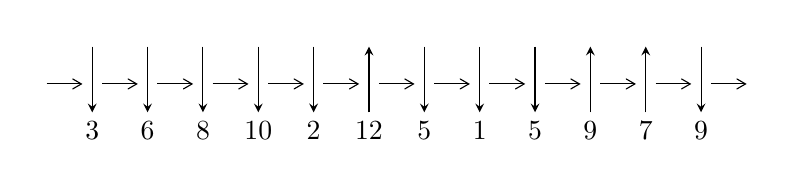
\begin{tikzpicture}[x=20pt, y=17pt]
	% nodes
	\node (C0) at (0, 0) {};
	\node (C1) at (1, 0) {};
	\node (C1U) at (1, +1) {};
	\node (C1D) at (1, -1) {3};

	\node (C2) at (2, 0) {};
	\node (C2U) at (2, +1) {};
	\node (C2D) at (2, -1) {6};

	\node (C3) at (3, 0) {};
	\node (C3U) at (3, +1) {};
	\node (C3D) at (3, -1) {8};

	\node (C4) at (4, 0) {};
	\node (C4U) at (4, +1) {};
	\node (C4D) at (4, -1) {10};

	\node (C5) at (5, 0) {};
	\node (C5U) at (5, +1) {};
	\node (C5D) at (5, -1) {2};

	\node (C6) at (6, 0) {};
	\node (C6U) at (6, +1) {};
	\node (C6D) at (6, -1) {12};

	\node (C7) at (7, 0) {};
	\node (C7U) at (7, +1) {};
	\node (C7D) at (7, -1) {5};

	\node (C8) at (8, 0) {};
	\node (C8U) at (8, +1) {};
	\node (C8D) at (8, -1) {1};

	\node (C9) at (9, 0) {};
	\node (C9U) at (9, +1) {};
	\node (C9D) at (9, -1) {5};

	\node (C10) at (10, 0) {};
	\node (C10U) at (10, +1) {};
	\node (C10D) at (10, -1) {9};

	\node (C11) at (11, 0) {};
	\node (C11U) at (11, +1) {};
	\node (C11D) at (11, -1) {7};

	\node (C12) at (12, 0) {};
	\node (C12U) at (12, +1) {};
	\node (C12D) at (12, -1) {9};
	\node (C13) at (13, 0) {};

	% arrows
	\draw[->,>={angle 60}]
	(C0) edge (C1) (C1) edge (C2) (C2) edge (C3) (C3) edge (C4) (C4) edge (C5) (C5) edge (C6) (C6) edge (C7) (C7) edge (C8) (C8) edge (C9) (C9) edge (C10) (C10) edge (C11) (C11) edge (C12) (C12) edge (C13) ;	\draw[->,>=stealth]
	(C1U) edge (C1D) (C2U) edge (C2D) (C3U) edge (C3D) (C4U) edge (C4D) (C5U) edge (C5D) (C6D) edge (C6U) (C7U) edge (C7D) (C8U) edge (C8D) (C9U) edge (C9D) (C10D) edge (C10U) (C11D) edge (C11U) (C12U) edge (C12D) ;
	\end{tikzpicture} \\
\hhline{~~} \\& 
\textbf{Solving Sequence} \\ \cline{2-2} 
 &
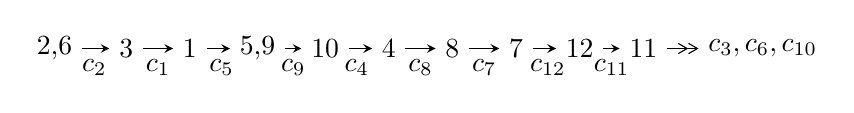
\begin{tikzpicture}[x=23pt, y=7pt]
	% node
	\node (A0) at (-1/8, 0) {2,6};
	\node (A1) at (1, 0) {3};
	\node (A2) at (2, 0) {1};
	\node (A3) at (49/16, 0) {5,9};
	\node (A4) at (33/8, 0) {10};
	\node (A5) at (41/8, 0) {4};
	\node (A6) at (49/8, 0) {8};
	\node (A7) at (57/8, 0) {7};
	\node (A8) at (65/8, 0) {12};
	\node (A9) at (73/8, 0) {11};
	\node (C1) at (1/2, -1) {$c_{2}$};
	\node (C2) at (3/2, -1) {$c_{1}$};
	\node (C3) at (5/2, -1) {$c_{5}$};
	\node (C4) at (29/8, -1) {$c_{9}$};
	\node (C5) at (37/8, -1) {$c_{4}$};
	\node (C6) at (45/8, -1) {$c_{8}$};
	\node (C7) at (53/8, -1) {$c_{7}$};
	\node (C8) at (61/8, -1) {$c_{12}$};
	\node (C9) at (69/8, -1) {$c_{11}$};
	\node (A10) at (11, 0) {$c_{3},c_{6},c_{10}$};

	% edge
	\draw[->,>=stealth]	
	(A0) edge (A1) (A1) edge (A2) (A2) edge (A3) (A3) edge (A4) (A4) edge (A5) (A5) edge (A6) (A6) edge (A7) (A7) edge (A8) (A8) edge (A9) ;
	\draw[->>,>={angle 60}]	
	(A9) edge (A10);
\end{tikzpicture} \\ 

\end{tabular} \\

\footnotetext{
The image of knot diagram is generated by the software ``\textbf{Draw programme}" developed by Andrew Bartholomew(\url{http://www.layer8.co.uk/maths/draw/index.htm\#Running-draw}), where we modified some parts for our purpose(\url{https://github.com/CATsTAILs/LinksPainter}).
}\phantom \\ \newline 
\centering \textbf{Ideals for irreducible components\footnotemark of $X_{\text{par}}$} 
 
\begin{align*}
I^u_{1}&=\langle 
-4 u^{23}+14 u^{22}+\cdots+b+7,\;-5 u^{24}+13 u^{23}+\cdots+2 a+6,\;u^{25}-5 u^{24}+\cdots+4 u-2\rangle \\
I^u_{2}&=\langle 
u^{15}-5 u^{13}-3 u^{12}+11 u^{11}+10 u^{10}-11 u^9-18 u^8+3 u^7+17 u^6+8 u^5-9 u^4-10 u^3-2 u^2+b+5 u+3,\\
\phantom{I^u_{2}}&\phantom{= \langle  }u^{15}-6 u^{13}-4 u^{12}+13 u^{11}+14 u^{10}-12 u^9-24 u^8- u^7+22 u^6+14 u^5-10 u^4-16 u^3-3 u^2+2 a+6 u+5,\\
\phantom{I^u_{2}}&\phantom{= \langle  }u^{16}+2 u^{15}+\cdots+3 u+2\rangle \\
I^u_{3}&=\langle 
- u^7 a-2 u^7+u^5 a- u^6+u^4 a+2 u^5-2 u^3 a+2 u^4- u^2 a-3 u^3- u^2+b+a+u+3,\\
\phantom{I^u_{3}}&\phantom{= \langle  }-2 u^7 a- u^6 a-3 u^7+2 u^5 a-2 u^6+3 u^4 a+4 u^5-2 u^3 a+5 u^4-2 u^2 a-5 u^3+a^2-5 u^2+3 a+3 u+6,\\
\phantom{I^u_{3}}&\phantom{= \langle  }u^8+u^7- u^6-2 u^5+u^4+2 u^3-2 u-1\rangle \\
\\
\end{align*}
\raggedright * 3 irreducible components of $\dim_{\mathbb{C}}=0$, with total 57 representations.\\
\footnotetext{All coefficients of polynomials are rational numbers. But the coefficients are sometimes approximated in decimal forms when there is not enough margin.}
\newpage
\renewcommand{\arraystretch}{1}
\centering \section*{I. $I^u_{1}= \langle -4 u^{23}+14 u^{22}+\cdots+b+7,\;-5 u^{24}+13 u^{23}+\cdots+2 a+6,\;u^{25}-5 u^{24}+\cdots+4 u-2 \rangle$}
\flushleft \textbf{(i) Arc colorings}\\
\begin{tabular}{m{7pt} m{180pt} m{7pt} m{180pt} }
\flushright $a_{2}=$&$\begin{pmatrix}1\\0\end{pmatrix}$ \\
\flushright $a_{6}=$&$\begin{pmatrix}0\\u\end{pmatrix}$ \\
\flushright $a_{3}=$&$\begin{pmatrix}1\\u^2\end{pmatrix}$ \\
\flushright $a_{1}=$&$\begin{pmatrix}- u^2+1\\- u^4\end{pmatrix}$ \\
\flushright $a_{5}=$&$\begin{pmatrix}u\\u\end{pmatrix}$ \\
\flushright $a_{9}=$&$\begin{pmatrix}\frac{5}{2} u^{24}-\frac{13}{2} u^{23}+\cdots-\frac{7}{2} u-3\\4 u^{23}-14 u^{22}+\cdots+3 u-7\end{pmatrix}$ \\
\flushright $a_{10}=$&$\begin{pmatrix}\frac{7}{2} u^{24}-\frac{23}{2} u^{23}+\cdots-\frac{13}{2} u+1\\u^{24}- u^{23}+\cdots+5 u^2-3\end{pmatrix}$ \\
\flushright $a_{4}=$&$\begin{pmatrix}-\frac{5}{2} u^{24}+\frac{21}{2} u^{23}+\cdots+\frac{13}{2} u-3\\-2 u^{24}+10 u^{23}+\cdots+7 u-5\end{pmatrix}$ \\
\flushright $a_{8}=$&$\begin{pmatrix}\frac{3}{2} u^{24}-\frac{17}{2} u^{23}+\cdots-\frac{13}{2} u+6\\-6 u^{24}+24 u^{23}+\cdots+13 u-7\end{pmatrix}$ \\
\flushright $a_{7}=$&$\begin{pmatrix}\frac{5}{2} u^{24}-\frac{11}{2} u^{23}+\cdots-\frac{3}{2} u-4\\-5 u^{24}+27 u^{23}+\cdots+18 u-17\end{pmatrix}$ \\
\flushright $a_{12}=$&$\begin{pmatrix}-\frac{3}{2} u^{24}+\frac{7}{2} u^{23}+\cdots+\frac{1}{2} u+3\\-2 u^{24}+5 u^{23}+\cdots+2 u+1\end{pmatrix}$ \\
\flushright $a_{11}=$&$\begin{pmatrix}-3 u^{24}+6 u^{23}+\cdots+2 u+6\\2 u^{24}-16 u^{23}+\cdots-11 u+14\end{pmatrix}$\\&\end{tabular}
\flushleft \textbf{(ii) Obstruction class $= -1$}\\~\\
\flushleft \textbf{(iii) Cusp Shapes $= -15 u^{24}+60 u^{23}-42 u^{22}-200 u^{21}+425 u^{20}+33 u^{19}-1003 u^{18}+891 u^{17}+934 u^{16}-2122 u^{15}+393 u^{14}+2207 u^{13}-1874 u^{12}-878 u^{11}+2018 u^{10}-425 u^9-1106 u^8+819 u^7+40 u^6-235 u^5+74 u^4-34 u^3+12 u^2+32 u-28$}\\~\\
\newpage\renewcommand{\arraystretch}{1}
\flushleft \textbf{(iv) u-Polynomials at the component}\newline \\
\begin{tabular}{m{50pt}|m{274pt}}
Crossings & \hspace{64pt}u-Polynomials at each crossing \\
\hline $$\begin{aligned}c_{1}\end{aligned}$$&$\begin{aligned}
&u^{25}+11 u^{24}+\cdots+12 u+4
\end{aligned}$\\
\hline $$\begin{aligned}c_{2},c_{5}\end{aligned}$$&$\begin{aligned}
&u^{25}+5 u^{24}+\cdots+4 u+2
\end{aligned}$\\
\hline $$\begin{aligned}c_{3},c_{4},c_{9}\end{aligned}$$&$\begin{aligned}
&u^{25}+19 u^{23}+\cdots+u+1
\end{aligned}$\\
\hline $$\begin{aligned}c_{6},c_{11}\end{aligned}$$&$\begin{aligned}
&u^{25}-18 u^{24}+\cdots-1792 u+256
\end{aligned}$\\
\hline $$\begin{aligned}c_{7}\end{aligned}$$&$\begin{aligned}
&u^{25}- u^{24}+\cdots+3881 u+1993
\end{aligned}$\\
\hline $$\begin{aligned}c_{8},c_{12}\end{aligned}$$&$\begin{aligned}
&u^{25}+u^{24}+\cdots+18 u+1
\end{aligned}$\\
\hline $$\begin{aligned}c_{10}\end{aligned}$$&$\begin{aligned}
&u^{25}-38 u^{24}+\cdots-7 u+1
\end{aligned}$\\
\hline
\end{tabular}\\~\\
\newpage\renewcommand{\arraystretch}{1}
\flushleft \textbf{(v) Riley Polynomials at the component}\newline \\
\begin{tabular}{m{50pt}|m{274pt}}
Crossings & \hspace{64pt}Riley Polynomials at each crossing \\
\hline $$\begin{aligned}c_{1}\end{aligned}$$&$\begin{aligned}
&y^{25}+9 y^{24}+\cdots+232 y-16
\end{aligned}$\\
\hline $$\begin{aligned}c_{2},c_{5}\end{aligned}$$&$\begin{aligned}
&y^{25}-11 y^{24}+\cdots+12 y-4
\end{aligned}$\\
\hline $$\begin{aligned}c_{3},c_{4},c_{9}\end{aligned}$$&$\begin{aligned}
&y^{25}+38 y^{24}+\cdots-7 y-1
\end{aligned}$\\
\hline $$\begin{aligned}c_{6},c_{11}\end{aligned}$$&$\begin{aligned}
&y^{25}+8 y^{24}+\cdots+393216 y-65536
\end{aligned}$\\
\hline $$\begin{aligned}c_{7}\end{aligned}$$&$\begin{aligned}
&y^{25}+59 y^{24}+\cdots+49162391 y-3972049
\end{aligned}$\\
\hline $$\begin{aligned}c_{8},c_{12}\end{aligned}$$&$\begin{aligned}
&y^{25}+33 y^{24}+\cdots+88 y-1
\end{aligned}$\\
\hline $$\begin{aligned}c_{10}\end{aligned}$$&$\begin{aligned}
&y^{25}-122 y^{24}+\cdots+73 y-1
\end{aligned}$\\
\hline
\end{tabular}\\~\\
\newpage\flushleft \textbf{(vi) Complex Volumes and Cusp Shapes}
$$\begin{array}{c|c|c}  
\text{Solutions to }I^u_{1}& \I (\text{vol} + \sqrt{-1}CS) & \text{Cusp shape}\\
 \hline 
\begin{aligned}
u &= -0.825841 + 0.556794 I \\
a &= -0.402690 - 0.517828 I \\
b &= -0.906052 - 0.019110 I\end{aligned}
 & \phantom{-}1.50077 + 2.23684 I & -2.22810 - 4.30531 I \\ \hline\begin{aligned}
u &= -0.825841 - 0.556794 I \\
a &= -0.402690 + 0.517828 I \\
b &= -0.906052 + 0.019110 I\end{aligned}
 & \phantom{-}1.50077 - 2.23684 I & -2.22810 + 4.30531 I \\ \hline\begin{aligned}
u &= \phantom{-}0.816024 + 0.629187 I \\
a &= \phantom{-}0.710669 + 1.151560 I \\
b &= \phantom{-}1.101890 + 0.658711 I\end{aligned}
 & \phantom{-}1.87514 + 0.07553 I & -5.11439 + 0.60620 I \\ \hline\begin{aligned}
u &= \phantom{-}0.816024 - 0.629187 I \\
a &= \phantom{-}0.710669 - 1.151560 I \\
b &= \phantom{-}1.101890 - 0.658711 I\end{aligned}
 & \phantom{-}1.87514 - 0.07553 I & -5.11439 - 0.60620 I \\ \hline\begin{aligned}
u &= \phantom{-}0.479269 + 0.953467 I \\
a &= \phantom{-}1.46509 + 0.67711 I \\
b &= -0.248526 + 0.073771 I\end{aligned}
 & \phantom{-}16.3921 - 2.3241 I & -0.96077 + 1.78819 I \\ \hline\begin{aligned}
u &= \phantom{-}0.479269 - 0.953467 I \\
a &= \phantom{-}1.46509 - 0.67711 I \\
b &= -0.248526 - 0.073771 I\end{aligned}
 & \phantom{-}16.3921 + 2.3241 I & -0.96077 - 1.78819 I \\ \hline\begin{aligned}
u &= \phantom{-}0.533110 + 0.937237 I \\
a &= -1.23338 - 1.32849 I \\
b &= \phantom{-}0.216650 - 0.151554 I\end{aligned}
 & \phantom{-}16.7595 + 7.3794 I & -1.22017 - 2.27864 I \\ \hline\begin{aligned}
u &= \phantom{-}0.533110 - 0.937237 I \\
a &= -1.23338 + 1.32849 I \\
b &= \phantom{-}0.216650 + 0.151554 I\end{aligned}
 & \phantom{-}16.7595 - 7.3794 I & -1.22017 + 2.27864 I \\ \hline\begin{aligned}
u &= \phantom{-}0.884641 + 0.632548 I \\
a &= -1.15580 - 0.83468 I \\
b &= -1.61829 - 0.44614 I\end{aligned}
 & \phantom{-}1.66131 - 5.01873 I & -5.13335 + 4.42111 I \\ \hline\begin{aligned}
u &= \phantom{-}0.884641 - 0.632548 I \\
a &= -1.15580 + 0.83468 I \\
b &= -1.61829 + 0.44614 I\end{aligned}
 & \phantom{-}1.66131 + 5.01873 I & -5.13335 - 4.42111 I\\
 \hline 
 \end{array}$$\newpage$$\begin{array}{c|c|c}  
\text{Solutions to }I^u_{1}& \I (\text{vol} + \sqrt{-1}CS) & \text{Cusp shape}\\
 \hline 
\begin{aligned}
u &= \phantom{-}1.130790 + 0.397647 I \\
a &= -0.250090 + 0.145886 I \\
b &= -0.517131 + 0.760870 I\end{aligned}
 & -3.90858 - 2.14605 I & -13.03933 - 1.76915 I \\ \hline\begin{aligned}
u &= \phantom{-}1.130790 - 0.397647 I \\
a &= -0.250090 - 0.145886 I \\
b &= -0.517131 - 0.760870 I\end{aligned}
 & -3.90858 + 2.14605 I & -13.03933 + 1.76915 I \\ \hline\begin{aligned}
u &= -1.106540 + 0.514773 I \\
a &= \phantom{-}0.501024 + 0.175726 I \\
b &= \phantom{-}0.976709 - 0.360023 I\end{aligned}
 & -3.10459 + 5.50284 I & -10.38958 - 5.97916 I \\ \hline\begin{aligned}
u &= -1.106540 - 0.514773 I \\
a &= \phantom{-}0.501024 - 0.175726 I \\
b &= \phantom{-}0.976709 + 0.360023 I\end{aligned}
 & -3.10459 - 5.50284 I & -10.38958 + 5.97916 I \\ \hline\begin{aligned}
u &= \phantom{-}0.751304\phantom{ +0.000000I} \\
a &= -0.162564\phantom{ +0.000000I} \\
b &= \phantom{-}0.399340\phantom{ +0.000000I}\end{aligned}
 & -0.992382\phantom{ +0.000000I} & -10.4670\phantom{ +0.000000I} \\ \hline\begin{aligned}
u &= -1.287770 + 0.035273 I \\
a &= -0.330208 + 1.190730 I \\
b &= -0.61690 + 2.67578 I\end{aligned}
 & \phantom{-}9.80615 + 5.07733 I & -5.58280 - 2.54938 I \\ \hline\begin{aligned}
u &= -1.287770 - 0.035273 I \\
a &= -0.330208 - 1.190730 I \\
b &= -0.61690 - 2.67578 I\end{aligned}
 & \phantom{-}9.80615 - 5.07733 I & -5.58280 + 2.54938 I \\ \hline\begin{aligned}
u &= -0.656789 + 0.222334 I \\
a &= \phantom{-}0.64095 + 1.30667 I \\
b &= \phantom{-}0.991318 + 0.792825 I\end{aligned}
 & -0.79508 - 1.66969 I & -0.88932 + 1.84897 I \\ \hline\begin{aligned}
u &= -0.656789 - 0.222334 I \\
a &= \phantom{-}0.64095 - 1.30667 I \\
b &= \phantom{-}0.991318 - 0.792825 I\end{aligned}
 & -0.79508 + 1.66969 I & -0.88932 - 1.84897 I \\ \hline\begin{aligned}
u &= \phantom{-}1.122380 + 0.708240 I \\
a &= \phantom{-}1.22419 + 0.85781 I \\
b &= \phantom{-}2.25460 + 1.97923 I\end{aligned}
 & \phantom{-}14.9497 - 13.4134 I & -3.26715 + 6.49403 I\\
 \hline 
 \end{array}$$\newpage$$\begin{array}{c|c|c}  
\text{Solutions to }I^u_{1}& \I (\text{vol} + \sqrt{-1}CS) & \text{Cusp shape}\\
 \hline 
\begin{aligned}
u &= \phantom{-}1.122380 - 0.708240 I \\
a &= \phantom{-}1.22419 - 0.85781 I \\
b &= \phantom{-}2.25460 - 1.97923 I\end{aligned}
 & \phantom{-}14.9497 + 13.4134 I & -3.26715 - 6.49403 I \\ \hline\begin{aligned}
u &= \phantom{-}1.155240 + 0.691095 I \\
a &= -0.673625 - 0.975766 I \\
b &= -1.24536 - 2.26158 I\end{aligned}
 & \phantom{-}14.3146 - 3.6962 I & -2.96996 + 2.38083 I \\ \hline\begin{aligned}
u &= \phantom{-}1.155240 - 0.691095 I \\
a &= -0.673625 + 0.975766 I \\
b &= -1.24536 + 2.26158 I\end{aligned}
 & \phantom{-}14.3146 + 3.6962 I & -2.96996 - 2.38083 I \\ \hline\begin{aligned}
u &= -0.120160 + 0.530735 I \\
a &= -0.414841 + 0.873103 I \\
b &= \phantom{-}0.411425 + 0.199437 I\end{aligned}
 & -0.69000 - 1.30270 I & -6.47181 + 4.99859 I \\ \hline\begin{aligned}
u &= -0.120160 - 0.530735 I \\
a &= -0.414841 - 0.873103 I \\
b &= \phantom{-}0.411425 - 0.199437 I\end{aligned}
 & -0.69000 + 1.30270 I & -6.47181 - 4.99859 I\\
 \hline 
 \end{array}$$\newpage\newpage\renewcommand{\arraystretch}{1}
\centering \section*{II. $I^u_{2}= \langle u^{15}-5 u^{13}+\cdots+b+3,\;u^{15}-6 u^{13}+\cdots+2 a+5,\;u^{16}+2 u^{15}+\cdots+3 u+2 \rangle$}
\flushleft \textbf{(i) Arc colorings}\\
\begin{tabular}{m{7pt} m{180pt} m{7pt} m{180pt} }
\flushright $a_{2}=$&$\begin{pmatrix}1\\0\end{pmatrix}$ \\
\flushright $a_{6}=$&$\begin{pmatrix}0\\u\end{pmatrix}$ \\
\flushright $a_{3}=$&$\begin{pmatrix}1\\u^2\end{pmatrix}$ \\
\flushright $a_{1}=$&$\begin{pmatrix}- u^2+1\\- u^4\end{pmatrix}$ \\
\flushright $a_{5}=$&$\begin{pmatrix}u\\u\end{pmatrix}$ \\
\flushright $a_{9}=$&$\begin{pmatrix}-\frac{1}{2} u^{15}+3 u^{13}+\cdots-3 u-\frac{5}{2}\\- u^{15}+5 u^{13}+\cdots-5 u-3\end{pmatrix}$ \\
\flushright $a_{10}=$&$\begin{pmatrix}\frac{1}{2} u^{15}+u^{14}+\cdots- u-\frac{1}{2}\\u^{14}+2 u^{13}+\cdots-3 u-1\end{pmatrix}$ \\
\flushright $a_{4}=$&$\begin{pmatrix}\frac{3}{2} u^{15}+2 u^{14}+\cdots+2 u+\frac{7}{2}\\- u^{15}- u^{14}+\cdots- u-3\end{pmatrix}$ \\
\flushright $a_{8}=$&$\begin{pmatrix}\frac{1}{2} u^{15}+u^{14}+\cdots-2 u-\frac{3}{2}\\u^{14}+u^{13}+\cdots-2 u-1\end{pmatrix}$ \\
\flushright $a_{7}=$&$\begin{pmatrix}-\frac{3}{2} u^{15}- u^{14}+\cdots-4 u-\frac{7}{2}\\-2 u^{15}- u^{14}+\cdots-4 u-3\end{pmatrix}$ \\
\flushright $a_{12}=$&$\begin{pmatrix}\frac{3}{2} u^{15}+2 u^{14}+\cdots+u+\frac{5}{2}\\2 u^{15}+2 u^{14}+\cdots+u+1\end{pmatrix}$ \\
\flushright $a_{11}=$&$\begin{pmatrix}3 u^{15}+4 u^{14}+\cdots+2 u+5\\4 u^{15}+4 u^{14}+\cdots+4 u+4\end{pmatrix}$\\&\end{tabular}
\flushleft \textbf{(ii) Obstruction class $= 1$}\\~\\
\flushleft \textbf{(iii) Cusp Shapes $= -3 u^{15}-4 u^{14}+8 u^{13}+15 u^{12}-12 u^{11}-29 u^{10}+5 u^9+35 u^8+7 u^7-27 u^6-22 u^5+10 u^4+16 u^3+3 u^2-11 u-10$}\\~\\
\newpage\renewcommand{\arraystretch}{1}
\flushleft \textbf{(iv) u-Polynomials at the component}\newline \\
\begin{tabular}{m{50pt}|m{274pt}}
Crossings & \hspace{64pt}u-Polynomials at each crossing \\
\hline $$\begin{aligned}c_{1}\end{aligned}$$&$\begin{aligned}
&u^{16}-8 u^{15}+\cdots-17 u+4
\end{aligned}$\\
\hline $$\begin{aligned}c_{2}\end{aligned}$$&$\begin{aligned}
&u^{16}+2 u^{15}+\cdots+3 u+2
\end{aligned}$\\
\hline $$\begin{aligned}c_{3},c_{9}\end{aligned}$$&$\begin{aligned}
&u^{16}+9 u^{14}+\cdots-4 u+1
\end{aligned}$\\
\hline $$\begin{aligned}c_{4}\end{aligned}$$&$\begin{aligned}
&u^{16}+9 u^{14}+\cdots+4 u+1
\end{aligned}$\\
\hline $$\begin{aligned}c_{5}\end{aligned}$$&$\begin{aligned}
&u^{16}-2 u^{15}+\cdots-3 u+2
\end{aligned}$\\
\hline $$\begin{aligned}c_{6}\end{aligned}$$&$\begin{aligned}
&u^{16}- u^{15}+\cdots- u+1
\end{aligned}$\\
\hline $$\begin{aligned}c_{7}\end{aligned}$$&$\begin{aligned}
&u^{16}+u^{15}+\cdots- u^2+1
\end{aligned}$\\
\hline $$\begin{aligned}c_{8}\end{aligned}$$&$\begin{aligned}
&u^{16}+u^{15}+\cdots+u+1
\end{aligned}$\\
\hline $$\begin{aligned}c_{10}\end{aligned}$$&$\begin{aligned}
&u^{16}-18 u^{15}+\cdots+4 u+1
\end{aligned}$\\
\hline $$\begin{aligned}c_{11}\end{aligned}$$&$\begin{aligned}
&u^{16}+u^{15}+\cdots+u+1
\end{aligned}$\\
\hline $$\begin{aligned}c_{12}\end{aligned}$$&$\begin{aligned}
&u^{16}- u^{15}+\cdots- u+1
\end{aligned}$\\
\hline
\end{tabular}\\~\\
\newpage\renewcommand{\arraystretch}{1}
\flushleft \textbf{(v) Riley Polynomials at the component}\newline \\
\begin{tabular}{m{50pt}|m{274pt}}
Crossings & \hspace{64pt}Riley Polynomials at each crossing \\
\hline $$\begin{aligned}c_{1}\end{aligned}$$&$\begin{aligned}
&y^{16}+4 y^{15}+\cdots-17 y+16
\end{aligned}$\\
\hline $$\begin{aligned}c_{2},c_{5}\end{aligned}$$&$\begin{aligned}
&y^{16}-8 y^{15}+\cdots-17 y+4
\end{aligned}$\\
\hline $$\begin{aligned}c_{3},c_{4},c_{9}\end{aligned}$$&$\begin{aligned}
&y^{16}+18 y^{15}+\cdots-4 y+1
\end{aligned}$\\
\hline $$\begin{aligned}c_{6},c_{11}\end{aligned}$$&$\begin{aligned}
&y^{16}+9 y^{15}+\cdots+5 y+1
\end{aligned}$\\
\hline $$\begin{aligned}c_{7}\end{aligned}$$&$\begin{aligned}
&y^{16}+15 y^{15}+\cdots-2 y+1
\end{aligned}$\\
\hline $$\begin{aligned}c_{8},c_{12}\end{aligned}$$&$\begin{aligned}
&y^{16}+5 y^{15}+\cdots+9 y+1
\end{aligned}$\\
\hline $$\begin{aligned}c_{10}\end{aligned}$$&$\begin{aligned}
&y^{16}-38 y^{15}+\cdots-60 y+1
\end{aligned}$\\
\hline
\end{tabular}\\~\\
\newpage\flushleft \textbf{(vi) Complex Volumes and Cusp Shapes}
$$\begin{array}{c|c|c}  
\text{Solutions to }I^u_{2}& \I (\text{vol} + \sqrt{-1}CS) & \text{Cusp shape}\\
 \hline 
\begin{aligned}
u &= -0.656997 + 0.743635 I \\
a &= -0.775458 + 1.141130 I \\
b &= -0.435041 + 0.316889 I\end{aligned}
 & \phantom{-}3.25303 - 1.48953 I & -2.71099 + 1.52251 I \\ \hline\begin{aligned}
u &= -0.656997 - 0.743635 I \\
a &= -0.775458 - 1.141130 I \\
b &= -0.435041 - 0.316889 I\end{aligned}
 & \phantom{-}3.25303 + 1.48953 I & -2.71099 - 1.52251 I \\ \hline\begin{aligned}
u &= -0.874191 + 0.334550 I \\
a &= -0.878721 - 0.189370 I \\
b &= -0.20139 - 1.91357 I\end{aligned}
 & \phantom{-}5.81030 + 1.43838 I & -3.56257 - 4.86268 I \\ \hline\begin{aligned}
u &= -0.874191 - 0.334550 I \\
a &= -0.878721 + 0.189370 I \\
b &= -0.20139 + 1.91357 I\end{aligned}
 & \phantom{-}5.81030 - 1.43838 I & -3.56257 + 4.86268 I \\ \hline\begin{aligned}
u &= \phantom{-}0.864296 + 0.625602 I \\
a &= \phantom{-}0.975538 - 0.892188 I \\
b &= \phantom{-}1.96131 + 0.43343 I\end{aligned}
 & \phantom{-}7.59435 - 2.44938 I & -5.19072 + 2.76813 I \\ \hline\begin{aligned}
u &= \phantom{-}0.864296 - 0.625602 I \\
a &= \phantom{-}0.975538 + 0.892188 I \\
b &= \phantom{-}1.96131 - 0.43343 I\end{aligned}
 & \phantom{-}7.59435 + 2.44938 I & -5.19072 - 2.76813 I \\ \hline\begin{aligned}
u &= \phantom{-}0.901146 + 0.140958 I \\
a &= -0.503170 + 1.005270 I \\
b &= -0.93293 + 1.12841 I\end{aligned}
 & -1.44134 + 1.66902 I & -13.69558 - 2.63152 I \\ \hline\begin{aligned}
u &= \phantom{-}0.901146 - 0.140958 I \\
a &= -0.503170 - 1.005270 I \\
b &= -0.93293 - 1.12841 I\end{aligned}
 & -1.44134 - 1.66902 I & -13.69558 + 2.63152 I \\ \hline\begin{aligned}
u &= -0.218755 + 0.798974 I \\
a &= \phantom{-}0.953181 - 0.233826 I \\
b &= -0.138155 + 0.327234 I\end{aligned}
 & \phantom{-}0.924346 - 0.806526 I & -1.176197 + 0.589571 I \\ \hline\begin{aligned}
u &= -0.218755 - 0.798974 I \\
a &= \phantom{-}0.953181 + 0.233826 I \\
b &= -0.138155 - 0.327234 I\end{aligned}
 & \phantom{-}0.924346 + 0.806526 I & -1.176197 - 0.589571 I\\
 \hline 
 \end{array}$$\newpage$$\begin{array}{c|c|c}  
\text{Solutions to }I^u_{2}& \I (\text{vol} + \sqrt{-1}CS) & \text{Cusp shape}\\
 \hline 
\begin{aligned}
u &= -1.002050 + 0.665576 I \\
a &= \phantom{-}1.051270 - 0.691243 I \\
b &= \phantom{-}1.76255 - 0.90512 I\end{aligned}
 & \phantom{-}2.21180 + 6.86626 I & -5.48184 - 7.08918 I \\ \hline\begin{aligned}
u &= -1.002050 - 0.665576 I \\
a &= \phantom{-}1.051270 + 0.691243 I \\
b &= \phantom{-}1.76255 + 0.90512 I\end{aligned}
 & \phantom{-}2.21180 - 6.86626 I & -5.48184 + 7.08918 I \\ \hline\begin{aligned}
u &= \phantom{-}1.165520 + 0.342736 I \\
a &= -0.333649 - 0.493333 I \\
b &= -0.168076 - 1.173650 I\end{aligned}
 & -3.25196 - 2.70217 I & -4.91112 + 4.04086 I \\ \hline\begin{aligned}
u &= \phantom{-}1.165520 - 0.342736 I \\
a &= -0.333649 + 0.493333 I \\
b &= -0.168076 + 1.173650 I\end{aligned}
 & -3.25196 + 2.70217 I & -4.91112 - 4.04086 I \\ \hline\begin{aligned}
u &= -1.178970 + 0.529446 I \\
a &= -0.238992 + 0.463717 I \\
b &= -0.84826 + 1.13723 I\end{aligned}
 & -1.94104 + 5.74574 I & -3.77099 - 5.59852 I \\ \hline\begin{aligned}
u &= -1.178970 - 0.529446 I \\
a &= -0.238992 - 0.463717 I \\
b &= -0.84826 - 1.13723 I\end{aligned}
 & -1.94104 - 5.74574 I & -3.77099 + 5.59852 I\\
 \hline 
 \end{array}$$\newpage\newpage\renewcommand{\arraystretch}{1}
\centering \section*{III. $I^u_{3}= \langle - u^7 a-2 u^7+\cdots+a+3,\;-2 u^7 a-3 u^7+\cdots+3 a+6,\;u^8+u^7- u^6-2 u^5+u^4+2 u^3-2 u-1 \rangle$}
\flushleft \textbf{(i) Arc colorings}\\
\begin{tabular}{m{7pt} m{180pt} m{7pt} m{180pt} }
\flushright $a_{2}=$&$\begin{pmatrix}1\\0\end{pmatrix}$ \\
\flushright $a_{6}=$&$\begin{pmatrix}0\\u\end{pmatrix}$ \\
\flushright $a_{3}=$&$\begin{pmatrix}1\\u^2\end{pmatrix}$ \\
\flushright $a_{1}=$&$\begin{pmatrix}- u^2+1\\- u^4\end{pmatrix}$ \\
\flushright $a_{5}=$&$\begin{pmatrix}u\\u\end{pmatrix}$ \\
\flushright $a_{9}=$&$\begin{pmatrix}a\\u^7 a+2 u^7+\cdots- a-3\end{pmatrix}$ \\
\flushright $a_{10}=$&$\begin{pmatrix}- u^7 a- u^7+u^5 a- u^6+u^5-2 u^3 a+2 u^4- u^3+a u- u^2+2 a+1\\u^7- u^4 a- u^5+u^2 a+2 u^3+a u- u-2\end{pmatrix}$ \\
\flushright $a_{4}=$&$\begin{pmatrix}- u^7 a-4 u^7+\cdots+2 a+7\\- u^7 a+u^5 a+u^6+u^4 a+2 u^5-2 u^3 a-3 u^3- u^2+a+u+1\end{pmatrix}$ \\
\flushright $a_{8}=$&$\begin{pmatrix}- u^6- u^3 a+u^4+u^3+a u+a-1\\u^7 a+2 u^7-2 u^5 a- u^4 a-2 u^5+2 u^3 a+u^2 a+4 u^3- a-2 u-3\end{pmatrix}$ \\
\flushright $a_{7}=$&$\begin{pmatrix}u^7+u^6- u^5-2 u^4+u^3+2 u^2-2\\u^7 a+3 u^7+\cdots-2 a-4\end{pmatrix}$ \\
\flushright $a_{12}=$&$\begin{pmatrix}u^7+u^6- u^5-2 u^4+u^3+2 u^2-2\\u^7 a+3 u^7+\cdots-2 a-4\end{pmatrix}$ \\
\flushright $a_{11}=$&$\begin{pmatrix}2 u^7+2 u^6-2 u^5-4 u^4+2 u^3+4 u^2-4\\2 u^7 a+6 u^7+\cdots-4 a-8\end{pmatrix}$\\&\end{tabular}
\flushleft \textbf{(ii) Obstruction class $= -1$}\\~\\
\flushleft \textbf{(iii) Cusp Shapes $= 4 u^7-8 u^5-4 u^4+8 u^3+4 u^2-4 u-6$}\\~\\
\newpage\renewcommand{\arraystretch}{1}
\flushleft \textbf{(iv) u-Polynomials at the component}\newline \\
\begin{tabular}{m{50pt}|m{274pt}}
Crossings & \hspace{64pt}u-Polynomials at each crossing \\
\hline $$\begin{aligned}c_{1}\end{aligned}$$&$\begin{aligned}
&(u^8+3 u^7+7 u^6+10 u^5+11 u^4+10 u^3+6 u^2+4 u+1)^2
\end{aligned}$\\
\hline $$\begin{aligned}c_{2},c_{5}\end{aligned}$$&$\begin{aligned}
&(u^8- u^7- u^6+2 u^5+u^4-2 u^3+2 u-1)^2
\end{aligned}$\\
\hline $$\begin{aligned}c_{3},c_{4},c_{9}\end{aligned}$$&$\begin{aligned}
&u^{16}+u^{15}+\cdots+344 u+313
\end{aligned}$\\
\hline $$\begin{aligned}c_{6},c_{11}\end{aligned}$$&$\begin{aligned}
&(u+1)^{16}
\end{aligned}$\\
\hline $$\begin{aligned}c_{7}\end{aligned}$$&$\begin{aligned}
&u^{16}- u^{15}+\cdots-400 u+617
\end{aligned}$\\
\hline $$\begin{aligned}c_{8},c_{12}\end{aligned}$$&$\begin{aligned}
&u^{16}-9 u^{15}+\cdots+62 u+23
\end{aligned}$\\
\hline $$\begin{aligned}c_{10}\end{aligned}$$&$\begin{aligned}
&u^{16}-27 u^{15}+\cdots-600312 u+97969
\end{aligned}$\\
\hline
\end{tabular}\\~\\
\newpage\renewcommand{\arraystretch}{1}
\flushleft \textbf{(v) Riley Polynomials at the component}\newline \\
\begin{tabular}{m{50pt}|m{274pt}}
Crossings & \hspace{64pt}Riley Polynomials at each crossing \\
\hline $$\begin{aligned}c_{1}\end{aligned}$$&$\begin{aligned}
&(y^8+5 y^7+11 y^6+6 y^5-17 y^4-34 y^3-22 y^2-4 y+1)^2
\end{aligned}$\\
\hline $$\begin{aligned}c_{2},c_{5}\end{aligned}$$&$\begin{aligned}
&(y^8-3 y^7+7 y^6-10 y^5+11 y^4-10 y^3+6 y^2-4 y+1)^2
\end{aligned}$\\
\hline $$\begin{aligned}c_{3},c_{4},c_{9}\end{aligned}$$&$\begin{aligned}
&y^{16}+27 y^{15}+\cdots+600312 y+97969
\end{aligned}$\\
\hline $$\begin{aligned}c_{6},c_{11}\end{aligned}$$&$\begin{aligned}
&(y-1)^{16}
\end{aligned}$\\
\hline $$\begin{aligned}c_{7}\end{aligned}$$&$\begin{aligned}
&y^{16}+39 y^{15}+\cdots+950600 y+380689
\end{aligned}$\\
\hline $$\begin{aligned}c_{8},c_{12}\end{aligned}$$&$\begin{aligned}
&y^{16}+7 y^{15}+\cdots+3424 y+529
\end{aligned}$\\
\hline $$\begin{aligned}c_{10}\end{aligned}$$&$\begin{aligned}
&y^{16}-53 y^{15}+\cdots-13866765616 y+9597924961
\end{aligned}$\\
\hline
\end{tabular}\\~\\
\newpage\flushleft \textbf{(vi) Complex Volumes and Cusp Shapes}
$$\begin{array}{c|c|c}  
\text{Solutions to }I^u_{3}& \I (\text{vol} + \sqrt{-1}CS) & \text{Cusp shape}\\
 \hline 
\begin{aligned}
u &= -0.570868 + 0.730671 I \\
a &= \phantom{-}0.748660 - 1.136300 I \\
b &= \phantom{-}0.218417 + 0.534766 I\end{aligned}
 & \phantom{-}5.53908 - 1.13123 I & \phantom{-}0.584775 + 0.510791 I \\ \hline\begin{aligned}
u &= -0.570868 + 0.730671 I \\
a &= -1.73857 + 0.97979 I \\
b &= -0.653022 + 0.489982 I\end{aligned}
 & \phantom{-}5.53908 - 1.13123 I & \phantom{-}0.584775 + 0.510791 I \\ \hline\begin{aligned}
u &= -0.570868 - 0.730671 I \\
a &= \phantom{-}0.748660 + 1.136300 I \\
b &= \phantom{-}0.218417 - 0.534766 I\end{aligned}
 & \phantom{-}5.53908 + 1.13123 I & \phantom{-}0.584775 - 0.510791 I \\ \hline\begin{aligned}
u &= -0.570868 - 0.730671 I \\
a &= -1.73857 - 0.97979 I \\
b &= -0.653022 - 0.489982 I\end{aligned}
 & \phantom{-}5.53908 + 1.13123 I & \phantom{-}0.584775 - 0.510791 I \\ \hline\begin{aligned}
u &= \phantom{-}0.855237 + 0.665892 I \\
a &= -0.019462 + 0.209322 I \\
b &= -1.39721 - 1.40003 I\end{aligned}
 & \phantom{-}8.73915 - 2.57849 I & \phantom{-}3.72292 + 3.56796 I \\ \hline\begin{aligned}
u &= \phantom{-}0.855237 + 0.665892 I \\
a &= \phantom{-}1.78204 - 1.77063 I \\
b &= \phantom{-}2.65743 - 0.64416 I\end{aligned}
 & \phantom{-}8.73915 - 2.57849 I & \phantom{-}3.72292 + 3.56796 I \\ \hline\begin{aligned}
u &= \phantom{-}0.855237 - 0.665892 I \\
a &= -0.019462 - 0.209322 I \\
b &= -1.39721 + 1.40003 I\end{aligned}
 & \phantom{-}8.73915 + 2.57849 I & \phantom{-}3.72292 - 3.56796 I \\ \hline\begin{aligned}
u &= \phantom{-}0.855237 - 0.665892 I \\
a &= \phantom{-}1.78204 + 1.77063 I \\
b &= \phantom{-}2.65743 + 0.64416 I\end{aligned}
 & \phantom{-}8.73915 + 2.57849 I & \phantom{-}3.72292 - 3.56796 I \\ \hline\begin{aligned}
u &= \phantom{-}1.09818\phantom{ +0.000000I} \\
a &= \phantom{-}0.054797 + 1.006860 I \\
b &= \phantom{-}0.67901 + 1.74126 I\end{aligned}
 & \phantom{-}0.0770056\phantom{ +0.000000I} & -5.86400\phantom{ +0.000000I} \\ \hline\begin{aligned}
u &= \phantom{-}1.09818\phantom{ +0.000000I} \\
a &= \phantom{-}0.054797 - 1.006860 I \\
b &= \phantom{-}0.67901 - 1.74126 I\end{aligned}
 & \phantom{-}0.0770056\phantom{ +0.000000I} & -5.86400\phantom{ +0.000000I}\\
 \hline 
 \end{array}$$\newpage$$\begin{array}{c|c|c}  
\text{Solutions to }I^u_{3}& \I (\text{vol} + \sqrt{-1}CS) & \text{Cusp shape}\\
 \hline 
\begin{aligned}
u &= -1.031810 + 0.655470 I \\
a &= -0.842370 + 0.591433 I \\
b &= -2.18592 + 0.93071 I\end{aligned}
 & \phantom{-}4.20006 + 6.44354 I & -1.42845 - 5.29417 I \\ \hline\begin{aligned}
u &= -1.031810 + 0.655470 I \\
a &= \phantom{-}0.99429 - 1.31993 I \\
b &= \phantom{-}1.27643 - 2.02437 I\end{aligned}
 & \phantom{-}4.20006 + 6.44354 I & -1.42845 - 5.29417 I \\ \hline\begin{aligned}
u &= -1.031810 - 0.655470 I \\
a &= -0.842370 - 0.591433 I \\
b &= -2.18592 - 0.93071 I\end{aligned}
 & \phantom{-}4.20006 - 6.44354 I & -1.42845 + 5.29417 I \\ \hline\begin{aligned}
u &= -1.031810 - 0.655470 I \\
a &= \phantom{-}0.99429 + 1.31993 I \\
b &= \phantom{-}1.27643 + 2.02437 I\end{aligned}
 & \phantom{-}4.20006 - 6.44354 I & -1.42845 + 5.29417 I \\ \hline\begin{aligned}
u &= -0.603304\phantom{ +0.000000I} \\
a &= -1.47939 + 1.27008 I \\
b &= -1.09513 - 1.46928 I\end{aligned}
 & \phantom{-}5.73470\phantom{ +0.000000I} & -3.89450\phantom{ +0.000000I} \\ \hline\begin{aligned}
u &= -0.603304\phantom{ +0.000000I} \\
a &= -1.47939 - 1.27008 I \\
b &= -1.09513 + 1.46928 I\end{aligned}
 & \phantom{-}5.73470\phantom{ +0.000000I} & -3.89450\phantom{ +0.000000I}\\
 \hline 
 \end{array}$$\newpage
\newpage\renewcommand{\arraystretch}{1}
\centering \section*{ IV. u-Polynomials}
\begin{tabular}{m{50pt}|m{274pt}}
Crossings & \hspace{64pt}u-Polynomials at each crossing \\
\hline $$\begin{aligned}c_{1}\end{aligned}$$&$\begin{aligned}
&(u^8+3 u^7+7 u^6+10 u^5+11 u^4+10 u^3+6 u^2+4 u+1)^2\\
&\cdot(u^{16}-8 u^{15}+\cdots-17 u+4)(u^{25}+11 u^{24}+\cdots+12 u+4)
\end{aligned}$\\
\hline $$\begin{aligned}c_{2}\end{aligned}$$&$\begin{aligned}
&((u^8- u^7+\cdots+2 u-1)^{2})(u^{16}+2 u^{15}+\cdots+3 u+2)\\
&\cdot(u^{25}+5 u^{24}+\cdots+4 u+2)
\end{aligned}$\\
\hline $$\begin{aligned}c_{3},c_{9}\end{aligned}$$&$\begin{aligned}
&(u^{16}+9 u^{14}+\cdots-4 u+1)(u^{16}+u^{15}+\cdots+344 u+313)\\
&\cdot(u^{25}+19 u^{23}+\cdots+u+1)
\end{aligned}$\\
\hline $$\begin{aligned}c_{4}\end{aligned}$$&$\begin{aligned}
&(u^{16}+9 u^{14}+\cdots+4 u+1)(u^{16}+u^{15}+\cdots+344 u+313)\\
&\cdot(u^{25}+19 u^{23}+\cdots+u+1)
\end{aligned}$\\
\hline $$\begin{aligned}c_{5}\end{aligned}$$&$\begin{aligned}
&((u^8- u^7+\cdots+2 u-1)^{2})(u^{16}-2 u^{15}+\cdots-3 u+2)\\
&\cdot(u^{25}+5 u^{24}+\cdots+4 u+2)
\end{aligned}$\\
\hline $$\begin{aligned}c_{6}\end{aligned}$$&$\begin{aligned}
&((u+1)^{16})(u^{16}- u^{15}+\cdots- u+1)(u^{25}-18 u^{24}+\cdots-1792 u+256)
\end{aligned}$\\
\hline $$\begin{aligned}c_{7}\end{aligned}$$&$\begin{aligned}
&(u^{16}- u^{15}+\cdots-400 u+617)(u^{16}+u^{15}+\cdots- u^2+1)\\
&\cdot(u^{25}- u^{24}+\cdots+3881 u+1993)
\end{aligned}$\\
\hline $$\begin{aligned}c_{8}\end{aligned}$$&$\begin{aligned}
&(u^{16}-9 u^{15}+\cdots+62 u+23)(u^{16}+u^{15}+\cdots+u+1)\\
&\cdot(u^{25}+u^{24}+\cdots+18 u+1)
\end{aligned}$\\
\hline $$\begin{aligned}c_{10}\end{aligned}$$&$\begin{aligned}
&(u^{16}-27 u^{15}+\cdots-600312 u+97969)(u^{16}-18 u^{15}+\cdots+4 u+1)\\
&\cdot(u^{25}-38 u^{24}+\cdots-7 u+1)
\end{aligned}$\\
\hline $$\begin{aligned}c_{11}\end{aligned}$$&$\begin{aligned}
&((u+1)^{16})(u^{16}+u^{15}+\cdots+u+1)(u^{25}-18 u^{24}+\cdots-1792 u+256)
\end{aligned}$\\
\hline $$\begin{aligned}c_{12}\end{aligned}$$&$\begin{aligned}
&(u^{16}-9 u^{15}+\cdots+62 u+23)(u^{16}- u^{15}+\cdots- u+1)\\
&\cdot(u^{25}+u^{24}+\cdots+18 u+1)
\end{aligned}$\\
\hline
\end{tabular}\newpage\renewcommand{\arraystretch}{1}
\centering \section*{ V. Riley Polynomials}
\begin{tabular}{m{50pt}|m{274pt}}
Crossings & \hspace{64pt}Riley Polynomials at each crossing \\
\hline $$\begin{aligned}c_{1}\end{aligned}$$&$\begin{aligned}
&(y^8+5 y^7+11 y^6+6 y^5-17 y^4-34 y^3-22 y^2-4 y+1)^2\\
&\cdot(y^{16}+4 y^{15}+\cdots-17 y+16)(y^{25}+9 y^{24}+\cdots+232 y-16)
\end{aligned}$\\
\hline $$\begin{aligned}c_{2},c_{5}\end{aligned}$$&$\begin{aligned}
&(y^8-3 y^7+7 y^6-10 y^5+11 y^4-10 y^3+6 y^2-4 y+1)^2\\
&\cdot(y^{16}-8 y^{15}+\cdots-17 y+4)(y^{25}-11 y^{24}+\cdots+12 y-4)
\end{aligned}$\\
\hline $$\begin{aligned}c_{3},c_{4},c_{9}\end{aligned}$$&$\begin{aligned}
&(y^{16}+18 y^{15}+\cdots-4 y+1)(y^{16}+27 y^{15}+\cdots+600312 y+97969)\\
&\cdot(y^{25}+38 y^{24}+\cdots-7 y-1)
\end{aligned}$\\
\hline $$\begin{aligned}c_{6},c_{11}\end{aligned}$$&$\begin{aligned}
&((y-1)^{16})(y^{16}+9 y^{15}+\cdots+5 y+1)\\
&\cdot(y^{25}+8 y^{24}+\cdots+393216 y-65536)
\end{aligned}$\\
\hline $$\begin{aligned}c_{7}\end{aligned}$$&$\begin{aligned}
&(y^{16}+15 y^{15}+\cdots-2 y+1)(y^{16}+39 y^{15}+\cdots+950600 y+380689)\\
&\cdot(y^{25}+59 y^{24}+\cdots+49162391 y-3972049)
\end{aligned}$\\
\hline $$\begin{aligned}c_{8},c_{12}\end{aligned}$$&$\begin{aligned}
&(y^{16}+5 y^{15}+\cdots+9 y+1)(y^{16}+7 y^{15}+\cdots+3424 y+529)\\
&\cdot(y^{25}+33 y^{24}+\cdots+88 y-1)
\end{aligned}$\\
\hline $$\begin{aligned}c_{10}\end{aligned}$$&$\begin{aligned}
&(y^{16}-53 y^{15}+\cdots-13866765616 y+9597924961)\\
&\cdot(y^{16}-38 y^{15}+\cdots-60 y+1)(y^{25}-122 y^{24}+\cdots+73 y-1)
\end{aligned}$\\
\hline
\end{tabular}
\vskip 2pc
\end{document}